% !TeX root = ../index.tex
\chapter{Sessions}
\graphicspath{{4-sessions/images/}}

\section{Exercise 1}

The code has been amended to properly display the widget order quantity on the confirmation page. This was the second most easiest method to implement as it only required starting a PHP Session in each of the scripts and using \texttt{\$\_SESSION} instead of \texttt{\$\_POST}.

Cookies are the hardest (but still straight forward) implement as a function is used to set the cookies using \texttt{setcookie(key, value)} and then using \texttt{\$\_COOKIE} instead of \texttt{\$\_POST} to access the value.

Hidden fields is the easiest method to implement as it only requires adding an extra field to the intermediary colour selection page that is hidden to the user.

\url{https://intweb.bucks.ac.uk/~21606555/oos/4-sessions/ex1.html}

\clearpage
\captionsetup{type=figure}\captionof{figure}{ex1.html}
\subfile{pyg/src/4-sessions/ex1}

\captionsetup{type=figure}\captionof{figure}{ex1-colour.php using session variables}
\subfile{pyg/src/4-sessions/ex1-colour}

\captionsetup{type=figure}\captionof{figure}{ex1-confirm.php using session variables}
\subfile{pyg/src/4-sessions/ex1-confirm}

\begin{figure}[H]
  \caption{Exercise 1 - Select quantity}
  \centering
  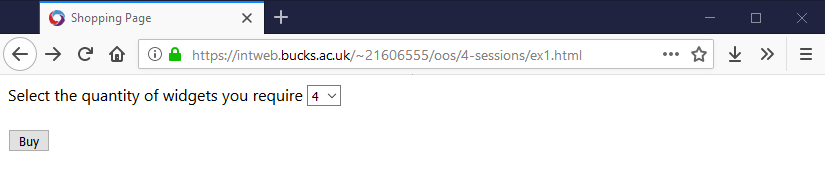
\includegraphics[width=\textwidth]{ex1-1quantity}
\end{figure}

\begin{figure}[H]
  \caption{Exercise 1 - Select colour}
  \centering
  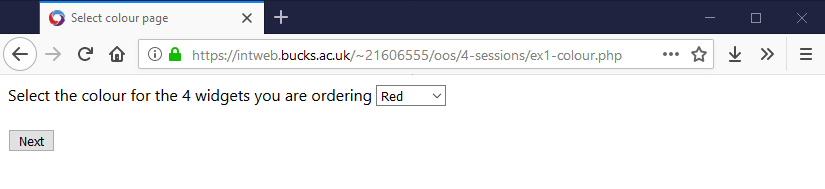
\includegraphics[width=\textwidth]{ex1-2colour}
\end{figure}

\begin{figure}[H]
  \caption{Exercise 1 - Result}
  \centering
  
\includegraphics[width=\textwidth]{ex1-3result}
\end{figure}

\section{Exercise 2}

Price has been added to \texttt{ex1.html} and stored as a session variable so it can be used on the confirmation page.

\url{https://intweb.bucks.ac.uk/~21606555/oos/4-sessions/ex2.html}

\captionsetup{type=figure}\captionof{figure}{ex2.html}
\subfile{pyg/src/4-sessions/ex2}

\clearpage
\captionsetup{type=figure}\captionof{figure}{ex2-colour.php setting price session variable}
\subfile{pyg/src/4-sessions/ex2-colour}

\captionsetup{type=figure}\captionof{figure}{ex2-confirm.php displaying price}
\subfile{pyg/src/4-sessions/ex2-confirm}

\begin{figure}[H]
  \caption{Exercise 2 - Select quantity}
  \centering
  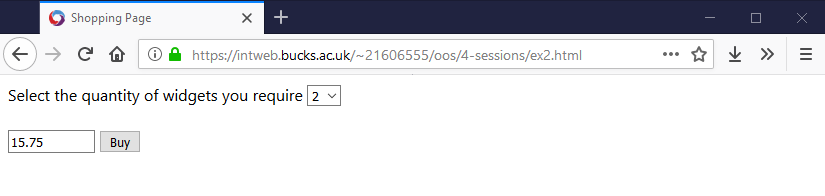
\includegraphics[width=\textwidth]{ex2-1quantity}
\end{figure}

\begin{figure}[H]
  \caption{Exercise 2 - Select colour}
  \centering
  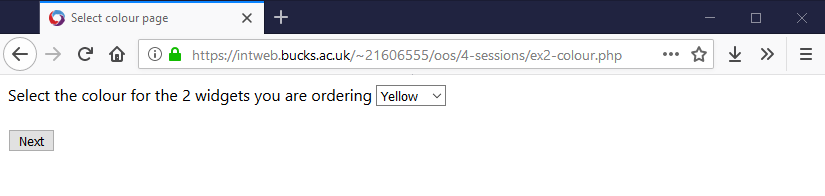
\includegraphics[width=\textwidth]{ex2-2colour}
\end{figure}

\begin{figure}[H]
  \caption{Exercise 2 - Result}
  \centering
  
\includegraphics[width=\textwidth]{ex2-3result}
\end{figure}

\clearpage
\section{Exercise 3}

The price has been removed from \texttt{ex3.html} and added to a new page \texttt{ex3-size.php}. This includes a dropdown to select the size of widgets. I decided to include the price in the dropdown (\texttt{Small (£15.75)}) which is then split when the data is stored in session variables. This avoids having to use a switch statement and keeps the sizing and pricing data in the same place for easier modification.

\url{https://intweb.bucks.ac.uk/~21606555/oos/4-sessions/ex3.html}

\captionsetup{type=figure}\captionof{figure}{ex3.html}
\subfile{pyg/src/4-sessions/ex3}

\clearpage
\captionsetup{type=figure}\captionof{figure}{ex3-size.php}
\subfile{pyg/src/4-sessions/ex3-size}

\clearpage
\captionsetup{type=figure}\captionof{figure}{ex3-colour.php}
\subfile{pyg/src/4-sessions/ex3-colour}

\captionsetup{type=figure}\captionof{figure}{ex3-confirm.php}
\subfile{pyg/src/4-sessions/ex3-confirm}

\begin{figure}[H]
  \caption{Exercise 3 - Select quantity}
  \centering
  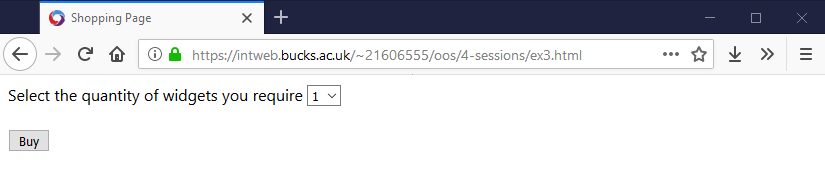
\includegraphics[width=\textwidth]{ex3-1quantity}
\end{figure}

\begin{figure}[H]
  \caption{Exercise 3 - Select size}
  \centering
  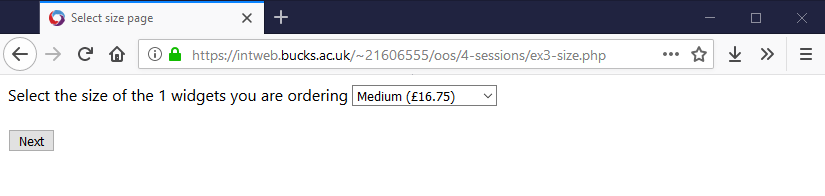
\includegraphics[width=\textwidth]{ex3-2size}
\end{figure}

\begin{figure}[H]
  \caption{Exercise 3 - Select colour}
  \centering
  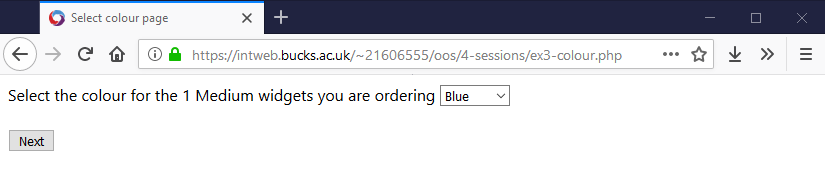
\includegraphics[width=\textwidth]{ex3-3colour}
\end{figure}

\begin{figure}[H]
  \caption{Exercise 3 - Result}
  \centering
  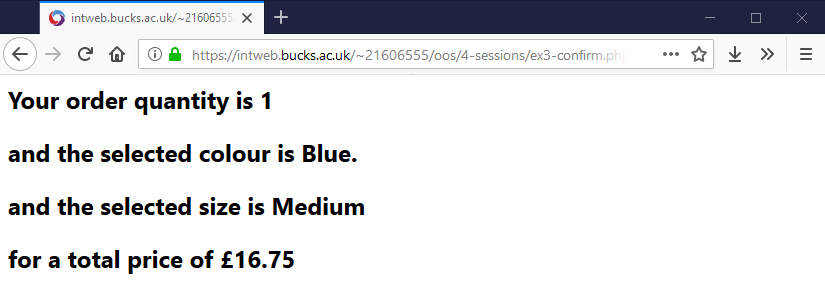
\includegraphics[width=\textwidth]{ex3-4result}
\end{figure}

\clearpage
\section{Exercise 4}

\begin{figure}[H]
  \caption{Exercise 4 - Order Form}
  \centering
  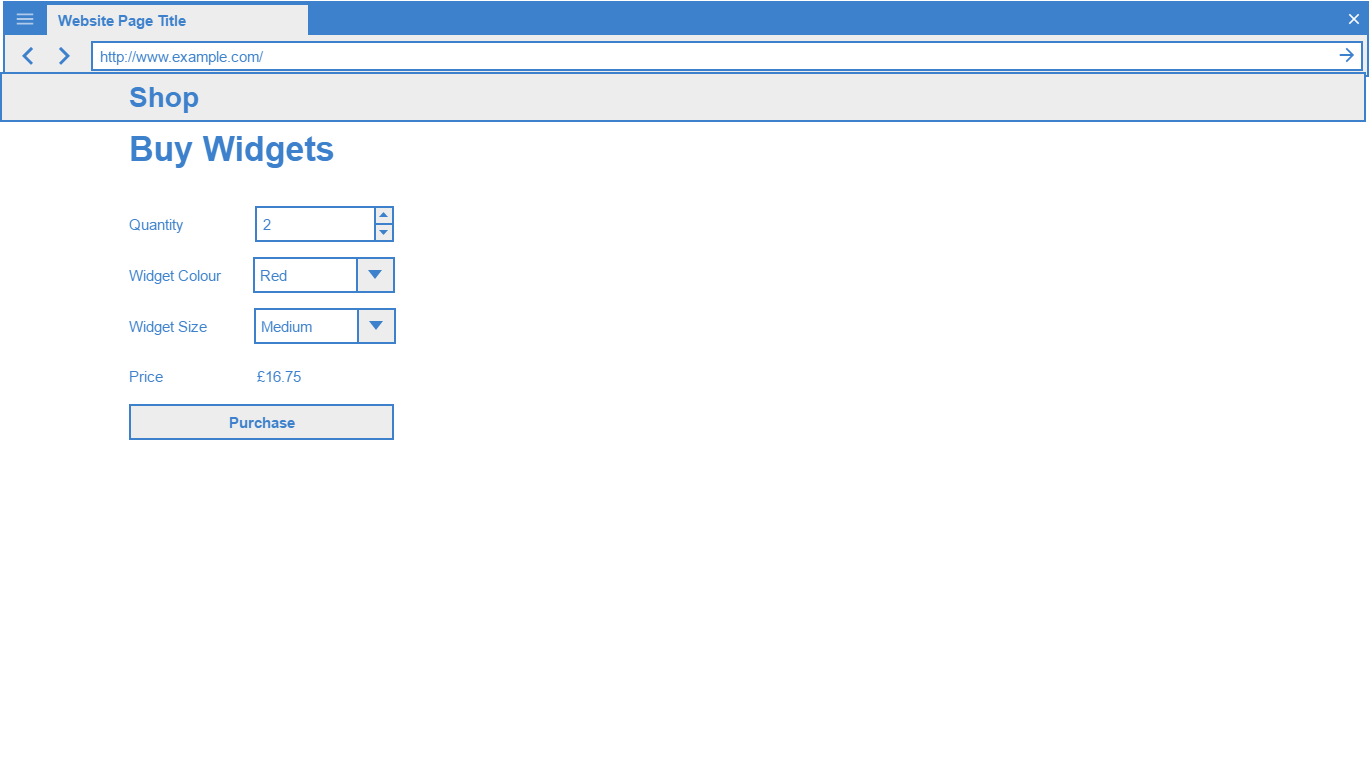
\includegraphics[width=\textwidth]{ex4-shop}
\end{figure}

\begin{figure}[H]
  \caption{Exercise 4 - Order Confirmation}
  \centering
  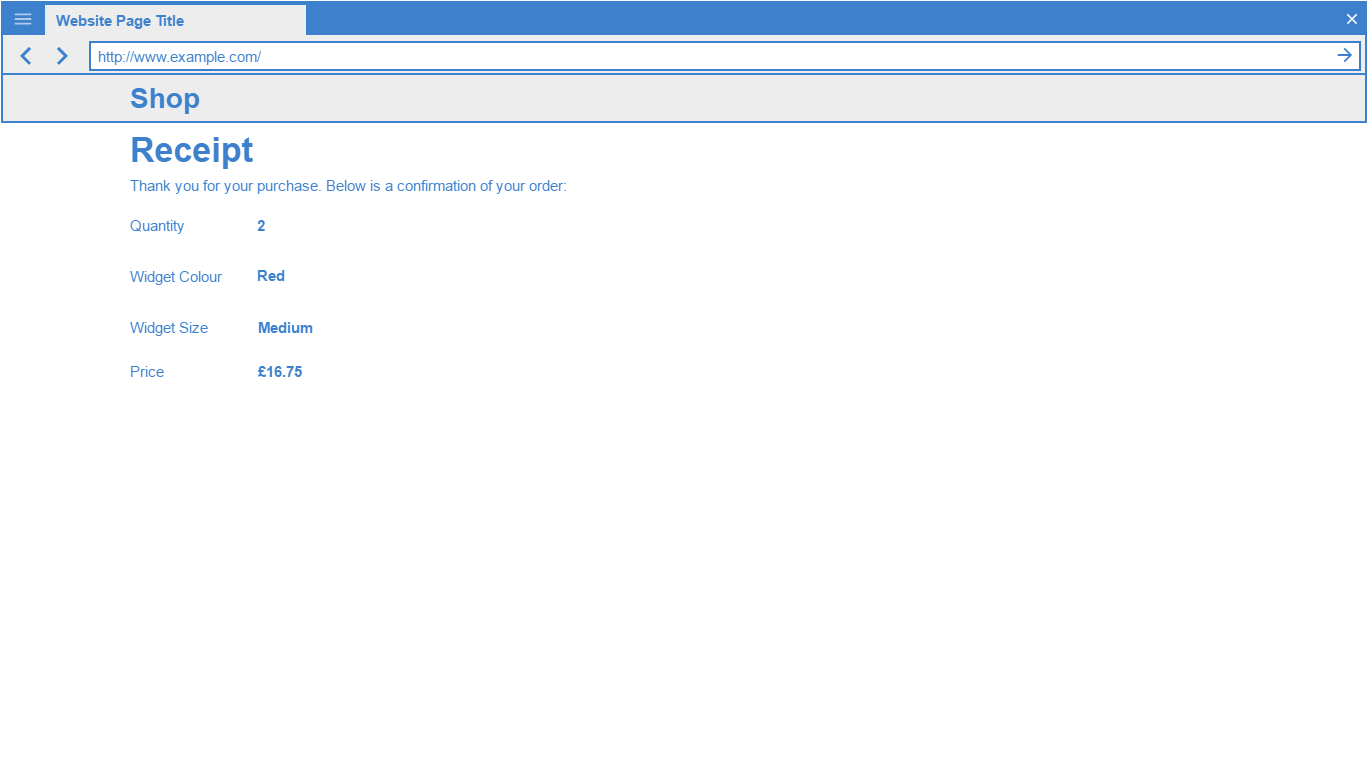
\includegraphics[width=\textwidth]{ex4-confirm}
\end{figure}
